\documentclass{article}
\usepackage{graphicx}
\usepackage{wrapfig}
\usepackage[margin=1in]{geometry}
\usepackage[font=small,labelfont=bf]{caption}


\graphicspath{{img/}{./img/}}
\setlength{\parindent}{10ex}

%
\title{\Large Population Heterogeneity in Efficient Coding of Natural Images}

\author{Vasha DuTell}

\date{}


\begin{document}

\maketitle


\section{Introduction}


	In Karklin and Simoncelli, 2011 \cite{karklin2011}, the authors train a linear/nonlinear neuron model on natural images with relatively simple constraints, and with the addition of gaussian noise, finding that this model learns the network of independently tiled on and off cell grids found in the retina. Here, I describe the biological and mathematical background underlying the model, and the significance of this result. I also describe my attempt to reproduce this finding, as well as my future work planned to extend this model into the time domain. \\


\section{Background}


\subsection{Efficient Coding Theory \& Mutual Information}


Efficient coding theory treats neural systems as optimized for the encoding of natural stimuli, constrained by efficiency of the encoding (Barlow, 1961). This type of model has been widely used in the literature to account for the circuitry seen in neural systems. One well known example is in sparse coding, a model constrained to maximizing fidelity of information encoding via reconstruction error, while minimizing metabolic cost. The power of this type of model is it allows coding schemes to be emerge naturally as a result of learning. If the model is subject to the same constraints as the brain, and the brain is indeed optimal, the model should converge on the same solution as the brain, resulting in great predictive power. \par
In quantifying efficiency, the metabolic cost of a neuron spiking is a key constraint, as the cost of spiking and neurotransmitter release accounts for 60-80 percent of the ATP used by a neuron \cite{FIND CITATION}. Given this high metabolic cost incurred by signaling, combined with evolutionary bottlenecks that have selected for minimizing metabolic cost in the organism as a whole, we expect neural systems may be optimized to to minimize overall spiking. Therefore, in efficient coding models, based on these assumptions, we constrain the model to minimize overall firing rate. \par
	Minimizing the firing rate of course, must be contrasted by another constraint, namely, the neural populations’ ability to perform some task useful to the organism. This is a more difficult constraint to define, and is in many ways up to one’s best guess at inferring the task a population of neurons is performing. Two educated guesses might be that the system is performing some computation, or perhaps faithfully transmitting information through a compressed channel, for use by downstream neurons. Here, we focus on the latter: faithful transmission of information along a limited set of wires, with as little information lost as possible. \par
Wishing to remain agnostic to the type of encoding the system may use, instead allowing our system to learn an efficient solution, we need a way to quantify information transmission without explicitly decoding the output of the network. We have a few options here. In an autoencoder framework, one could add an additional layer to the output layer, and train the network to reconstruct the input signal, penalizing reconstruction error. Alternatively, and the approach taken in this paper, is to use a measure from information theory which requires only probability distributions to calculate, mutual information. Mutual information is defined as the difference between the entropy of the input $X$ and the conditional entropy of the input given the response $R$:  $I(X;R) = H(X) - H(X|R)$. These values can be measured without explicitly knowing the encoding, allowing us to constrain a model to maximize this value, making it a useful quantity with which to constrain the model. \par


\subsection{Retinal anatomy - on and off cells}
	In the visual system, the transmission of visual information from the retina in the eye to the Lateral Geniculate Nucleus (LGN) through the optic nerve is an example of an information bottleneck, where the signal must be efficiently compressed in order to faithfully transmit information to the brain for further processing. In transmitting the visual signal from the retina to the brain, the visual system splits the signal along two separate channels. One neuron type, ‘On-center’ ganglion cells increase spiking in response to light in in the center of the receptive field, while ‘Off-center’ neurons respond to lack of light in the center of their receptive field. If we treat this encoding as optimal from an efficient coding perspective, we can assume that this choice to split the signal is an efficient coding strategy that helps to maximize the transmitted information to the brain from the retina. In this case, a model of this system that is constrained in the same way should reproduce this split. \par


\section{Karklin \& Simoncelli Model}


\subsection{Model Description}

\begin{wrapfigure}{2}{0.4\linewidth}
  \centering
    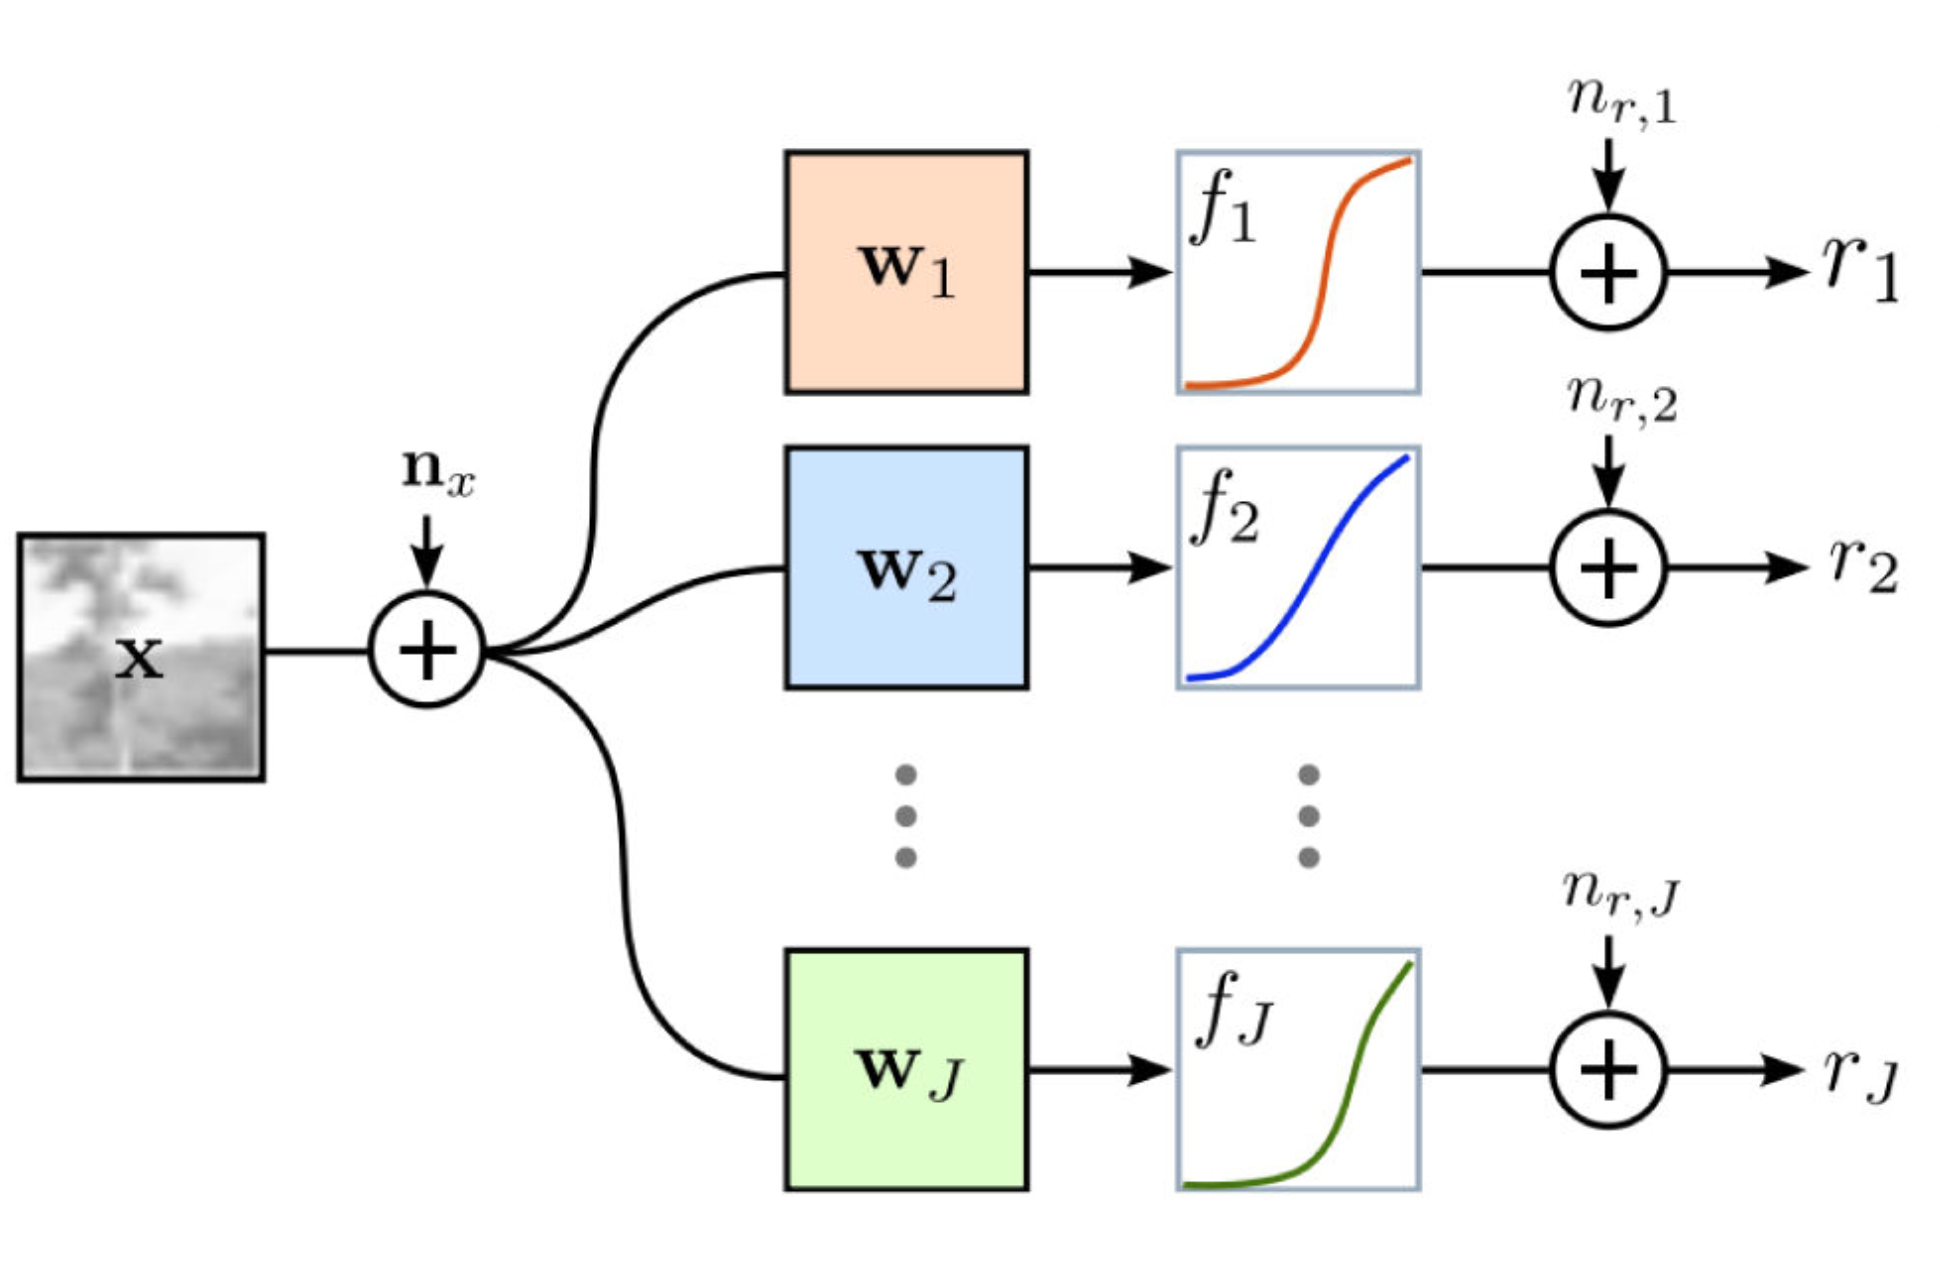
\includegraphics[width=1\linewidth]{ksfig1.png}
  \caption{Linear-Nonlinear Model {\cite{karksim11}}).}
  \label{fig:ksfig1}
\end{wrapfigure}

In Karlin \& Simoncelli, 2011, early visual system is modeled \cite{karklin2011} using a set of linear/nonlinear neurons which encode the image patches, compressing them from a 256-D space to a 100-D space, in a manner reminiscent of the retina. In the model  \ref{fig:ksfig1}, natural image patches $x$ are combined with static Gaussian noise $n_x$. Linear weights $w$ are trained, which in turn feed to nonlinear functions $g$. Finally, output noise $n_r$ is added, combined with an offset $f_o$ and responses $r$ measured \ref{fig:karksim11}. In the paper, nonlinear functions are learned in addition to the weights. These nonlinear functions are parameterized as mixtures of 500 Gaussians, so that the shape of the resulting activation curve can be learned. The response of each neuron $i$ is calculated as:
$$r^i \approx \textbf{G}^i \textbf{W}^T (x^i+n_x^i)+n_r^i + f_o^i$$




Where the nonlinear responses are approximated to first-order Taylor approximation by $\textbf{G}^i$, a diagonal matrix where each diagonal entry is the response of each nonlinear function at the output $y$ from the filters $W$,  $g(y)$. \par
The model is trained using gradient ascent to maximize an objective function embodying efficiency, maximizing mutual information between the image and the response $I(X;R)$, while minimizing the overall spiking rate of the output $<r_j>$. These two quantities are weighted together using the function $\lambda$ as a tradeoff parameter, adjusted to achieve an average response value $r$ of one per neuron per image. Because the global input entropy $H(X)$ is does not depend on the model, mutual information is maximized by maximizing as negative conditional entropy $-H(X|R)$. \par


$$ max(I(X;R) - \sum_j{\lambda_j <r_j>}) $$
$$ max(H(X)-H(X|R) - \sum_j{\lambda_j <r_j>}) $$
$$ max(-H(X|R) - \sum_j{\lambda_j <r_j>}) $$


The conditional entropy is calculated using the determinant of the covariance matrix  of the posterior distribution $C_{x|r}, p(x|r)$. The posterior is in turn calculated by the covariance of the prior $C_{r|x}, p(r|x)$, multiplied by the weights $W$ and the diagonal matrix of the nonlinear responses $G$, and added to the inverse of the global covariance matrix of the input images $C_x$. This is in turn calculated by combining the global covariance of the images $C_x$, the weights $W$, the slope of the activation function for a given image $G$, as well as the covariances of the input noise $C_nx$ and of the response noise $C_{nr}$. \par


$$ max(-H(X|R) = -E[\frac{1}{2} ln 2 \pi e det(\textbf{C}^i_{x|r})]) $$


$$ \textbf{C}^i_{x|r} = (\textbf{C}_{x}^{-1} + \textbf{W} \textbf{G}^i (\textbf{C}^{i_{r|x}})^{-1} \textbf{G}^i \textbf{W}^T )^{i^{-1}} $$


$$ \textbf{C}^i_{r|x} = \textbf{G}^i \textbf{W}^T \textbf{C}_{n_x} \textbf{W} \textbf{G}^i  + \textbf{C}_{n_r} $$




\subsection{Original Results}


\begin{wrapfigure}{2}{0.4\linewidth}
  \centering
    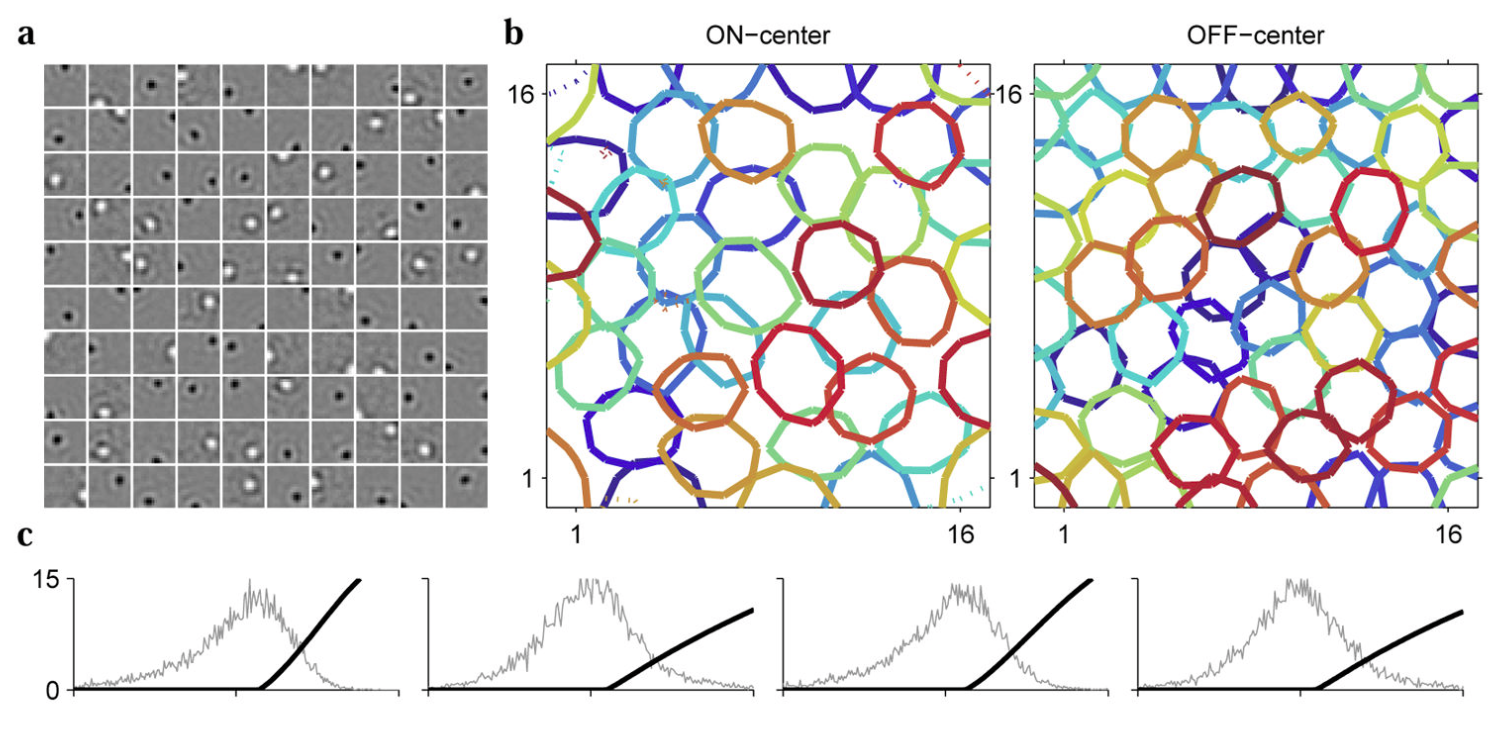
\includegraphics[width=1\linewidth]{ksfig2.png}
  \caption{Expected Results {\cite{karksim11}}).}
  \label{fig:ksfig2}
\end{wrapfigure}

After training, expected results are weights learned such that the entire stimulus space is tiled by the filters. In the regime of little noise in the input and output (20dB), this algorithm collapses to simply reproduce ICA, and the resulting receptive fields are composed of mostly homogeneous gaborlets tiling the input space. However, in the presence of increasing noise (8bD input, -6dB response), the weights split into heterogeneous populations, with the two populations independently tiling. This population split in in the responses, with one population responding to high activation (bright), and the other population to low activation (dark). This parallels the population split that we see in biological visual systems, particularly in retinal ganglion cells, implying that this model may well represent the structure and constraints underlying this small part of the visual system. This model learning to encode visual information in the same way the visual system has with such a simple model with few constants is what makes this paper so incredible. \par
The second main finding is in learning the activation functions. While they are constrained only to be positive and monotonically increasing, the network learned hard rectifier activation functions, and with rectification positioned near the mode of the filter output. This is consistent with literature suggesting though soft rectification is more common in neurons, hard rectification is more useful in the presence of noise \cite{Caradini}. A final finding surrounds the value of $\lambda$ needed to produce an average firing rate of 1 per neuron per image patch. This implies that the system imparts an information gain of 20 bits with its compression. \par


\section{Reproducing Model \& Results}


\subsection{Model Differences}
My implementation of this model runs in TensorFlow, with a few differences in implementation. First, I do not simulate the activation functions as mixtures of gaussians, instead learning for each neuron more simply an offset and a slope for a rectified linear function. This of course means that the sharp rectification is pre-defined rather than learned, but the offsets and slopes of the response functions can still be learned. The more complicated mixture of 500 Gaussians per neuron as described in the paper can be added later, but at the moment I have bigger problems (see next section). \par
As a result of the simpler relu with a learned offset and slope that I use as compared to the original model, I do not need to use $\textbf{G}$ to make the first-order Taylor approximation of the in the calculation of the response function. I can instead directly calculate the response using the relu function with a given slope and offset. \par
A final difference between my model and the original implementation is I that use a different natural scene database. I use the vanHateren Natural Image Database \cite{VanHateren}. However, it is still a natural scene database, grayscaled, with mean and variance normalized to 1 at the full image level, and then split into 16x16 patches in the same way. I expect this different database should not make a difference in my result, though the paper specified that the images were linear with respect to light levels, and I’m not sure if this is true with the vanHateren images dataset I’m using. \par



\subsection{Conclusions and Why I Might be Running into Problems}

\begin{wrapfigure}{1}{0.4\linewidth}
  \centering
    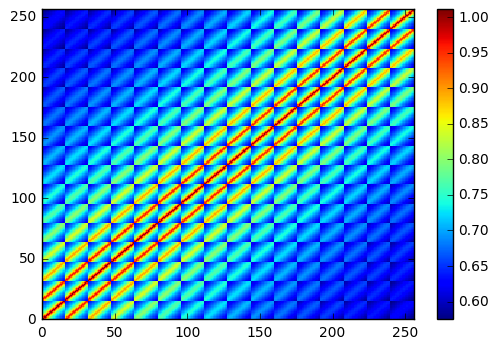
\includegraphics[width=1\linewidth]{covx.png}
  \caption{Covariance Matrix of Input}
  \label{fig:covx}
\end{wrapfigure}

There is currently a problem with the training in my implementation, where the firing rate will change to increase the objective function, but the information will not change. The problem is related to the calculation of the $C_{x|r}$ term, which when the determinant of this matrix is calculated in the equation for $H(X|R)$, evaluates at zero. This results in a constant near zero value for the information. Mathematically speaking, for a square matrix, there are only a few potential reasons for a zero determinant. Either an entire row is zero, two rows or columns are equal, or a row or column is a multiple of another. Computationally rather than mathematically however, there is another potential cause of a zero determinant.  If the values in the matrix are so small that when they are multiplied together, they become evaluated at zero by the computer. Given the small numbers in these matrices, I suspect this is the underlying problem. \par
	I believe that the root of the problem may lie in $C_x$, the covariance matrix of the input images having too small values. I have checked this calculation multiple times and $C_x$ appears as expected \cite{fig:covx}, but perhaps it may need to be normalized in some other way. In order to test this, I used the trace of $C_x$ to approximate the determinant of $C_x$ in the calculation of mutual information. The trace is the derivative of the determinant of a matrix, and is the sum of a matrix’s eigenvalues, while the determinant is the product of the eigenvalues. Clearly they are not equivalent, but are related enough that in the absence of other options, I can at least use the trace to get some result. \par

\begin{wrapfigure}{2}{0.4\linewidth}
  \centering
    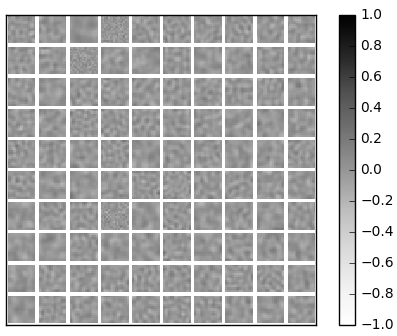
\includegraphics[width=1\linewidth]{traceresults.png}
  \caption{My Results using Tr($C_{x|r})$}
  \label{fig:traceresults}
\end{wrapfigure}

Using the trace, I was able to get a change in the information, and for some semblance of receptive fields to emerge, validating that my model can learn. However, the model still cannot learn properly. The receptive fields gained from this different but related model are not even Gabor patches \cite{fig:traceresults}. \par
	Another potential cause of this error could be due to an initialization of the response functions. If they were too low, this would cause the matrix G to be mostly the zero matrix, resulting in a very small $C_{x|r}$ However, I don't think this is very likely because if this were the case, using the trace instead would still result in the same zero determinant. I have also experimented with changing noise values from very low to very high, as well as the initialization weights, and offsets, and slopes for the relus, to no avail. I think that makes this possibility unlikely.\par
	One misunderstanding I initially had with the model was I expected the input and output noises to be of a constant distribution, but varied with each image and each trial. When i implemented the model this way I was unable to learn anything, and only when I appreciated this difference was I able to train using the trace. I believe this is an important limitation of this model, as I believe it more biologically plausible for noise to change, otherwise it is not much different than an offset. \par


\section{Future work - Extension into Time Domain}


Future goals of this work (after of course getting it to work as-is) are to extend the model into the time domain, by modifying this model to take in a natural movie, and optimizing an information rate between the input and response. Like the spatial patterns in natural scenes that influence visual system’s choice to split into on and off cells, spatio-temporal patterns in natural movies may lead to another population split, given the correct objective function and constraints.  \par
In the time domain, one hint at a potential split to expect is in the temporal response properties of neurons. In the mammalian visual system,visual signal is split between M and P ganglion cells, which have complementary responses to the spatio-temporal spectrum. M (parasol) ganglion cells have large receptive fields with fast temporal response properties, while  P (midge) ganglion cells have small receptive fields with slower temporal response properties. If this split is an efficient coding strategy, such a model of efficient coding in the time domain may reproduce this. \par




\section{References}


%\bibliographystyle{{plain}
{\footnotesize \bibliography{mybib}}





\end{document}





